
\section{\name{} Dataset}
\label{sec:dataset_creation}

Our dataset, \name{}, aims to offer a robust evaluation benchmark for physical commonsense in video generative models. Specifically, the dataset is curated with guidelines to cover (a) a wide range of daily activities and objects in the physical world (e.g., rolling objects, pouring liquid into a glass), (b) physical interactions between various material types (e.g., solid-solid or solid-fluid interactions), and (c) the perceived complexity of rendering objects and motions under graphic simulation. For instance, \textit{ketchup}, which follows non-newtonian fluid dynamics \cite{witczak2011non}, is harder to model and simulate than \textit{water}, which follows newtonian fluid dynamics, using traditional fluid simulators \cite{bridson2015fluid}. Under the collection guidelines, we curate a list of text prompts that will be used for conditioning the text-to-video generative models. Specifically, we follow the 3-stage pipeline to create the dataset.


\begin{table}[h]
\centering
\begin{tabular}{ccl}
\hline
\textbf{Category}    & \textbf{Difficulty} & \textbf{Example Captions}                                                                                                              \\\hline
\multirow{1}{*}[-0.6em]{Solid-Solid} & Easy       & \begin{tabular}[c]{@{}l@{}}Bottle topples off the table. (\explain{rigid bodies})\end{tabular}              \\\cline{2-3}
& Hard       & \begin{tabular}[c]{@{}l@{}}Scrubber scrubs a dirty dish. (\explain{complex contacts})\end{tabular}                \\\hline
\multirow{1}{*}[-0.6em]{Solid-Fluid} & Easy       & \begin{tabular}[c]{@{}l@{}}Water flows down a circular drain. (\explain{contacts with rigid bodies})\end{tabular}     \\\cline{2-3}
& Hard       & \begin{tabular}[c]{@{}l@{}}A swimmer splashing in the sea water. (\explain{contacts with high-speed})\end{tabular} \\\hline
\multirow{1}{*}[-0.6em]{Fluid-Fluid} & Easy       & \begin{tabular}[c]{@{}l@{}}Rain splashing on a pond. (\explain{mixing of same fluids})\end{tabular}              \\\cline{2-3}
& Hard       & \begin{tabular}[c]{@{}l@{}}Ink spreading in still water. (\explain{mixing of different fluids})\end{tabular} \\\hline       
\end{tabular}
\caption{\small{\textbf{Example captions in the \name{} dataset.} Specifically, we design them to depict the interactions between two states of matter (solid-solid, solid-fluid, fluid-fluid). We further classify the captions as easy or hard based on the modeling and simulation complexity in the computer graphics. We highlight the reasoning behind the easy and hard annotations by our expert annotators in the \explain{()}.}}
\label{tab:example}
\end{table}

\paragraph{LLM-Generated Captions (Stage 1).} Here, we query a large language model, in our case GPT-4 \cite{gpt4}, to generate a list of $1000$ \textit{candidate} captions depicting real-world dynamics. As the majority of real-world dynamics involve solids or fluids, we broadly classify those dynamics into three categories: \textit{solid-solid} interactions, \textit{solid-fluid} interactions, and \textit{fluid-fluid} interactions. Specifically, we consider fluid dynamics involving in-viscid and viscous flows—representative examples being water and honey, respectively. On the other hand, we find that solids exhibit more diverse constitutive models, including but not limited to rigid bodies, elastic materials, sands, metals, and snow. In total, we prompt GPT-4 to generate $500$ candidate captions for solid-solid and solid-fluid interactions, and $200$ candidate captions for fluid-fluid interactions. We present the GPT-4 prompts in Appendix \ref{app:interaction_specific_prompts}.  

\paragraph{Human Verification (Stage 2).} Since LLM-generated captions may not adhere to our input query, we perform a human verification step to filter bad generations. Specifically, the authors perform human verification to ensure the quality and relevance of the captions, adhering to these criteria: (1) the caption must be clear and understandable; (2) the caption should avoid excessive complexity, such as overly varied objects or too intricate dynamics; and (3) the captions must accurately reflect the intended interaction categories (e.g., that fluids are mentioned in solid-fluid or fluid-fluid dynamics). 
% To maintain focus on the fundamental interactions among solids and fluids, we also exclude captions involving complex physical phenomena such as phase changes (e.g. ice melting into water) or magnetic effects. \hb{Tianyi, add content here based on NeurIPS rebuttal.} 
Finally, we have $688$ captions where $289$ captions for solid-solid interactions, $291$ for solid-fluid interactions, and $108$ for fluid-fluid interactions, respectively. We highlight that our prompts include a wide range of material types and physical interactions that are common in both real life and the graphics community. Material types include simple rigid bodies \cite{liang2018gpu}, deformable bodies \cite{huang2021plasticinelab}, think shells \cite{chen2018physical}, metal \cite{li2022energetically}, fracture \cite{wolper2020anisompm}, cream \cite{yue2015continuum}, sand \cite{klar2016drucker} and so on. The contact handling is also diverse as it is based on the interactions of all aforementioned materials \cite{gu2023maniskill2, li2020incremental, han2023convex, zong2024convex}. \hb{Data quality is paramount for evaluating foundation models. For instance, Winoground (400 examples) \cite{thrush2022winoground}, Visit-Bench (500 examples) \cite{bitton2023visit}, LLaVA-Bench (90 examples) \cite{liu2024visual}, and Vibe-Eval (269 examples) \cite{padlewski2024vibe} are commonly employed to assess vision-language models due to their high-quality despite their limited size. Given that human verification demands significant expert hours and is not scalable within our budget, we prioritize data quality for evaluating T2V models.}


\begin{figure}[t!]
% \vspace{-5mm}
 \begin{minipage}{0.45\textwidth} 
 \centering
 \captionof{table}{Statistics of the \name{} dataset.}
 \label{tab:statistics}
\begin{tabular}{ccc}\toprule
\textbf{Statistic} &\textbf{Number} \\\hline

Total captions & $688$ \\
Unique actions & $138$ \\
Total T2V models & $\hb{12}$ \\
Total generated videos & $\hb{11330}$ \\
\hline
Human annotations & $\hb{36500}$ \\ 
\hline
Category (Interacting materials)  &3 \\
Solid-Solid &289 \\
Solid-Fluid &291 \\
Fluid-Fluid &108 \\\hline
Category (Interaction complexity) & 2 \\
Easy & $366$ \\
Hard & $322$ \\
% \hline
% Average length of caption &8.5 \\
\bottomrule
\end{tabular}
 \end{minipage} 
 \hfill
 \begin{minipage}{0.5\textwidth}
 \centering
 % \vspace{-1mm}
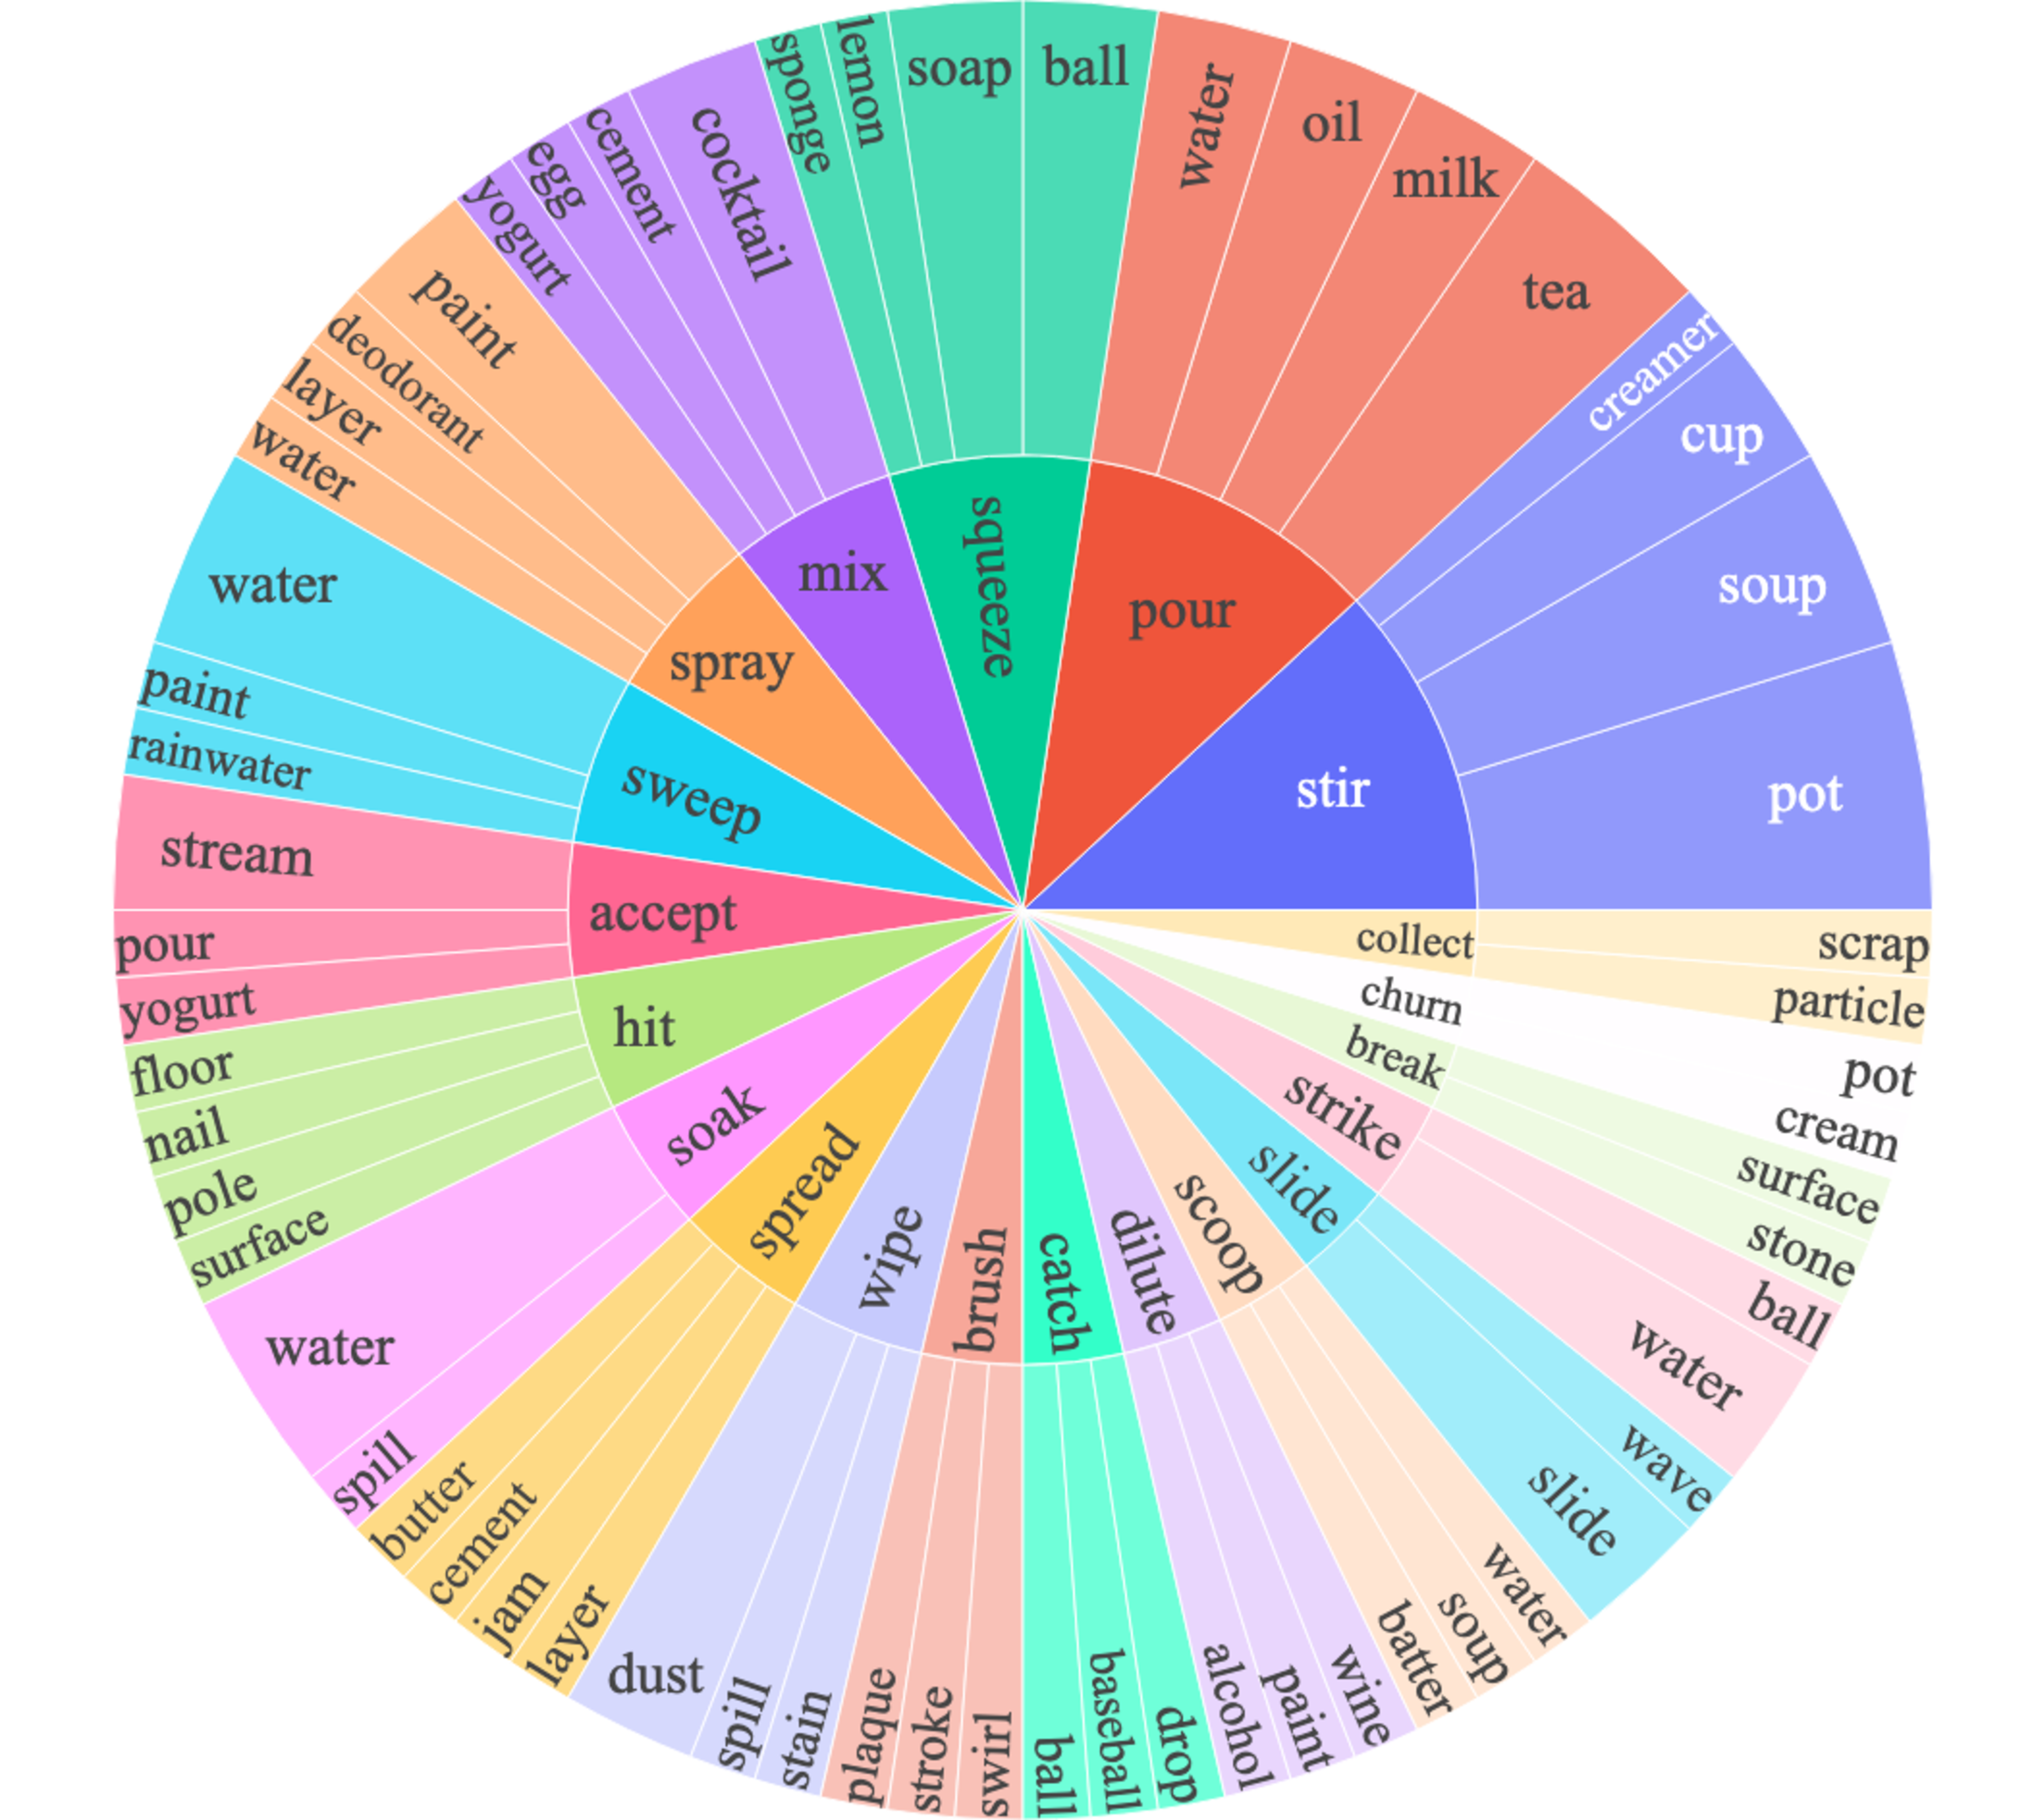
\includegraphics[width=0.8\textwidth]{images/all_wheel.pdf}
% \vspace{-1mm}
 \caption{\small{Top-20 most frequently occurring verbs (inner) and their top-4 direct nouns (outer) in captions.}}
 \label{fig:source_dataset}
 \end{minipage}
 % \vspace{-2mm}
\end{figure}



\paragraph{Difficulty Annotation (Stage 3).} To acquire fine-grained insights into the quality of the video generation, we further annotate our each instance in the dataset with perceived \textit{difficulty}. Specifically, we ask two experienced graphics researchers (senior Ph.D. students in physics-based simulation) to independently classify each caption as easy (0) or hard (1) based on their perception of the complexity in simulating the objects and motions in the captions using state-of-the-art physics engines \cite{li2020incremental, chen2023multi, xie2023contact, zong2023neural, qu2023power, fang2020iq}. Subsequently, the disagreements were discussed to reach a unanimous judgment for less than $5\%$ of the instances.
\tx{The difficulty of a simulation is primarily influenced by the complexity of the model, which varies depending on the type of material. For example, deformable bodies pose a greater modeling challenge than rigid bodies because they change shape under external forces, leading to more complex partial differential equations (PDEs). In contrast, rigid bodies maintain their shape, resulting in simpler models. Another key factor is the numerical difficulty in solving these equations, which increases with the material's velocity, especially when high-order terms are involved in the PDEs. As a result, slower-moving materials are generally easier to simulate than faster-moving ones.} 
We note that the level of difficulty is evaluated within each category (e.g., solid-solid, solid-fluid, fluid-fluid), and cannot be compared across different categories. We present the examples for generated captions in Table \ref{tab:example}.
% in Appendix \ref{app:example_captions}.





\paragraph{Data Analysis.} A fine-grained metadata facilitates a comprehensive understanding of the benchmark. Specifically, we present the main statistics of the \name{} dataset in Table \ref{tab:statistics}. Notably, we generate $11330$ videos for the prompts in the dataset using a diverse range of generative models. In addition, the average caption length is $8.5$ words, indicating that most captions are straightforward and do not complicate our analysis with complex phrasing that could be excessively challenging the generative models. \footnote{\hb{We use GPT-4 to enhance and generate longer versions of the original captions. However, we found that most of the T2V models are poor at following long/enhanced captions most of the time.}} The dataset includes 138 unique actions grounded in our captions. Figure \ref{fig:source_dataset} visualizes the root verbs and direct nouns used in the \name{} captions, highlighting the diversity of actions and entities. Hence, our dataset encompasses a wide range of visual concepts and actions. We perform fine-grained diversity analysis in Appendix \ref{sec:fine-wheel}.
